\chapter{Diseño del Simulador}
\label{cap:diseno}

En este capítulo se presenta la arquitectura del simulador de códigos BCH desarrollado, detallando las decisiones de diseño, la organización de los componentes y el flujo de información.

\section{Especificación de Requisitos y Funcionalidades}

\subsection{Requisitos Funcionales}

\begin{itemize}
    \item \textbf{RF1.} Aritmética completa en el cuerpo finito $GF(2^m)$ mediante tablas log/antilog.
    \item \textbf{RF2.} Configuración flexible de parámetros $(m, t)$ con cálculo automático de $n$ y $k$.
    \item \textbf{RF3.} Codificación sistemática mediante construcción del polinomio generador.
    \item \textbf{RF4.} Simulación de canales BSC y AWGN con modulación BPSK (decisión dura).
    \item \textbf{RF5.} Decodificación algebraica completa (síndromes, Berlekamp-Massey y búsqueda de Chien).
    \item \textbf{RF6.} Soporte para procesamiento de ficheros reales.
    \item \textbf{RF7.} Recolección y exportación de métricas (BER, BER uncoded, CWER y tiempos).
\end{itemize}

\subsection{Requisitos No Funcionales}
Los requisitos no funcionales definen las restricciones y atributos de calidad del sistema:
\begin{itemize}
    \item \textbf{RNF1. Rendimiento}: Procesar millones de palabras código en tiempos razonables mediante optimizaciones de bajo nivel y paralelización.
    \item \textbf{RNF2. Modularidad y Reusabilidad}: Separación clara entre álgebra, códec y simulación.
    \item \textbf{RNF3. Reproducibilidad}: Resultados deterministas cuando se fija una semilla.
    \item \textbf{RNF4. Mantenibilidad}: Código bien documentado y orientado a objetos.
    \item \textbf{RNF5. Limitaciones aceptadas}: Soporte hasta $m=15$, solo decodificación \textit{hard-decision}.
\end{itemize}
    
\section{Diseño del Sistema}
Se ha diseñado el software bajo un enfoque modular, facilitando la validación independiente de la lógica matemática y de la lógica de simulación.

\subsection{Arquitectura}
La estructura se divide en tres niveles de abstracción:

\begin{enumerate}
    \item \textbf{Capa de Álgebra:} Contiene las abstracciones matemáticas de elementos del Cuerpo y polinomios.
    \item \textbf{Capa de Aplicación (BCH):} Contiene el protocolo de codificación y decodificación, utilizando los servicios de la capa de álgebra.
    \item \textbf{Capa de Simulación:} Contiene el proceso de generación de ruido estadístico, la paralelización por hilos y la recolección de métricas de rendimiento.
\end{enumerate}
\begin{figure}[ht]
    \centering
    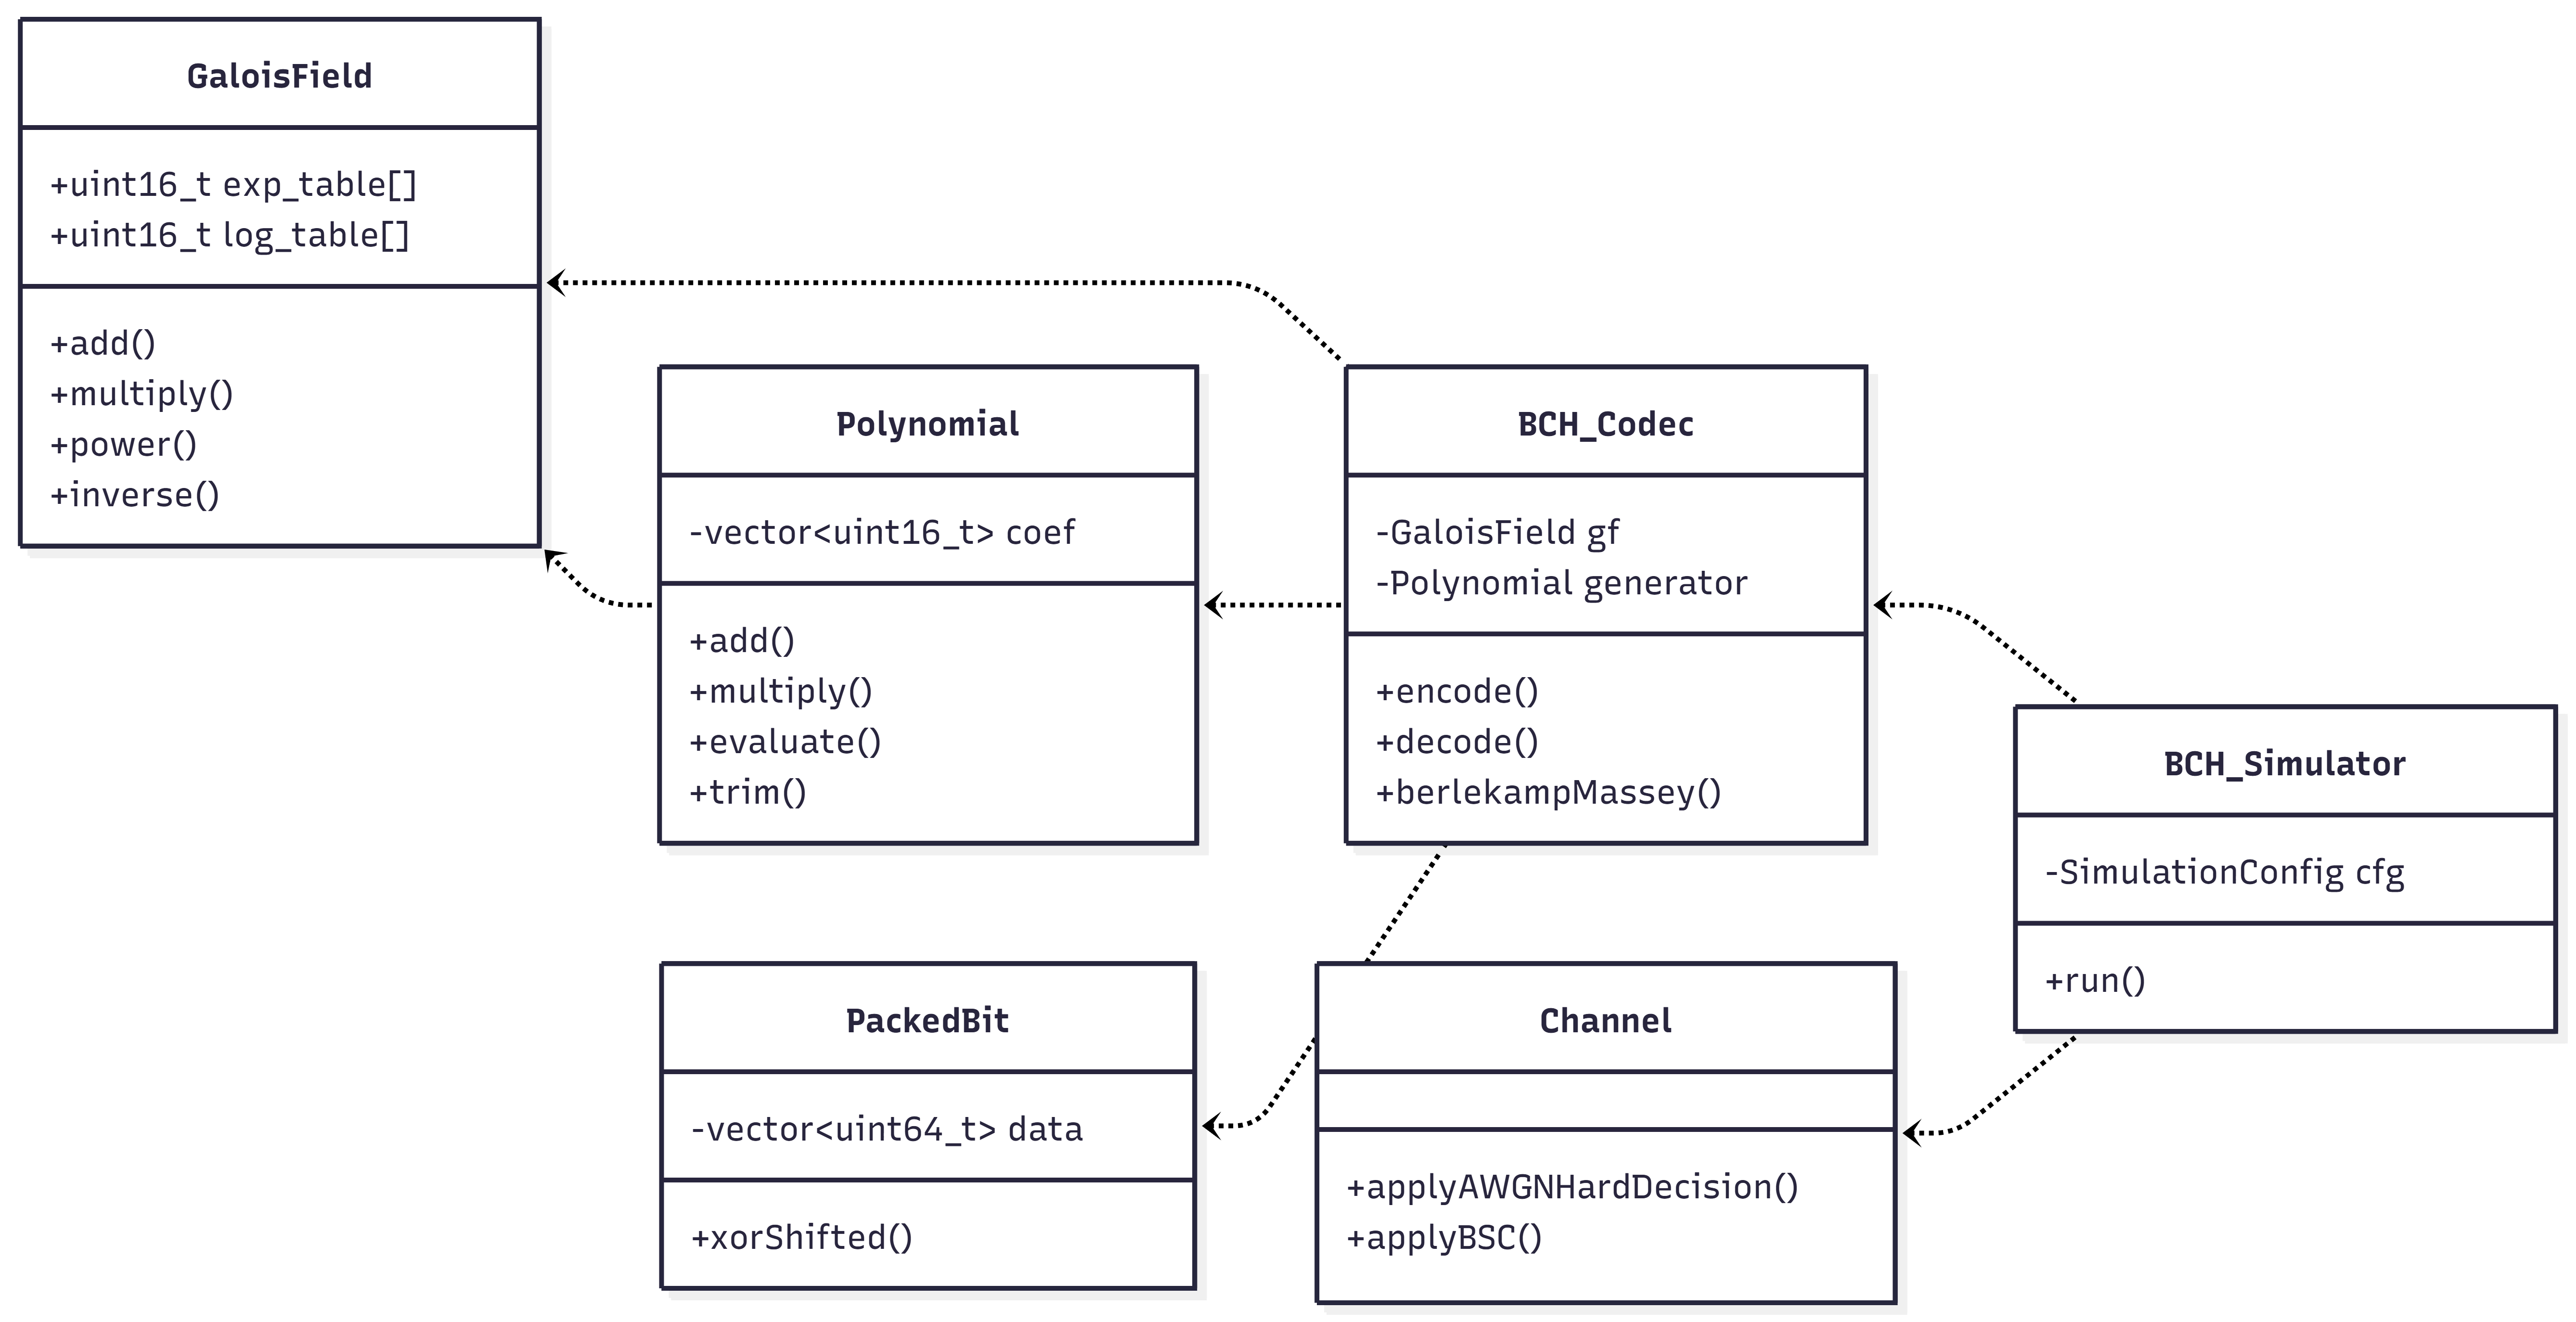
\includegraphics[width=0.95\textwidth]{../imagenes/UML_general.png}
    \caption{Diagrama de clases UML general del simulador BCH.}
    \label{fig:uml_general}
\end{figure}
\subsection{Flujo de Información y Modelo de Simulación}

El simulador sigue un esquema de procesamiento paralelo por palabra código, aprovechando la independencia entre simulaciones Monte Carlo. 

A diferencia de un enfoque secuencial, el diseño distribuye la carga de trabajo mediante \textbf{OpenMP}, donde cada hilo ejecuta de forma autónoma el ciclo completo: generación del mensaje → codificación → paso por el canal → decodificación → recolección de errores.

En la Figura \ref{fig:diagrama_flujo_paralelo} se muestra este flujo paralelo. La configuración global inicializa las tablas estáticas del Cuerpo de Galois una única vez. Posteriormente, el \texttt{BCH\_Simulator} lanza un pool de hilos que ejecutan de manera independiente el pipeline de simulación. Los resultados se sincronizan al final para calcular las métricas agregadas (BER, CWER, tiempos, etc.).
\begin{figure}[h]
    \centering
    \shorthandoff{>}
    \resizebox{\textwidth}{!}{
    \begin{tikzpicture}[
        node distance=1cm,
        block/.style={draw, rounded corners, minimum width=2.5cm, minimum height=1cm, align=center, font=\small},
        thread/.style={draw, dashed, gray, rounded corners, inner sep=10pt},
        arrow/.style={thick, ->, >=stealth}
    ]

    % Bloque inicial
    \node[block] (config) {Configuración\\y Tablas Log/Exp};
    % Representación de Paralelismo (Threads)
    \node[block, below=1.5cm of config] (enc1) {Codificación};
    \node[block, left=0.5cm of enc1] (enc0) {Codificación};
    \node[block, right=0.5cm of enc1] (enc2) {Codificación};
    
    \node[block, below=1.2cm of enc1] (canal1) {Canal\\(AWGN/BSC)};
    \node[block, left=0.5cm of canal1] (canal0) {Canal\\(AWGN/BSC)};
    \node[block, right=0.5cm of canal1] (canal2) {Canal\\(AWGN/BSC)};

    \node[block, below=1.2cm of canal1] (dec1) {Decodificación\\(B-M / Chien)};
    \node[block, left=0.5cm of dec1] (dec0) {Decodificación\\(B-M / Chien)};
    \node[block, right=0.5cm of dec1] (dec2) {Decodificación\\(B-M / Chien)};
    % Bloque final de reducción
    \node[block, below=1.5cm of dec1] (metrics) {Sincronización\\y Métricas (CSV)};
    % Caja que indica paralelismo
    \node[thread, fit=(enc0) (enc2) (dec0) (dec2), label=right:{\small Paralelismo OpenMP}] (pool) {};
    % Flechas
    \draw[arrow] (config) -- (pool.north);
    \draw[arrow] (enc0) -- (canal0); \draw[arrow] (canal0) -- (dec0);
    \draw[arrow] (enc1) -- (canal1); \draw[arrow] (canal1) -- (dec1);
    \draw[arrow] (enc2) -- (canal2); \draw[arrow] (canal2) -- (dec2);
    \draw[arrow] (pool.south) -- (metrics);
    \end{tikzpicture}
    }
    \shorthandon{>} 
    \caption{Flujo de información paralelo para simulación de Monte Carlo.}
    \label{fig:diagrama_flujo_paralelo}
\end{figure}

\subsection{Diseño de Datos y Estructuras}
\label{sub:diseno_datos}

Para conseguir un buen equilibrio entre rendimiento y claridad del código, se han tomado las siguientes decisiones clave de representación de datos:
\begin{itemize}
    \item \textbf{Elementos del cuerpo y coeficientes polinómicos:} Utilización de \verb|uint16_t| (suficiente para $m \leq 15$) para mejorar la localidad de memoria y el uso de caché.
    
    \item \textbf{Optimización de operaciones bit a bit:} La clase \texttt{PackedBit} permite realizar desplazamientos y XOR en bloques de 64 bits, fundamental para acelerar la división polinómica en la codificación sistemática.
    
    \item \textbf{Cuerpo de Galois:} Tablas \texttt{exp\_table} y \texttt{log\_table} declaradas como \textbf{estáticas}, calculándose una sola vez por valor de $m$.

    \item \textbf{Polinomios:} Representados mediante \texttt{std::vector<uint16\_t>} con método \texttt{trim()} para eliminar coeficientes nulos de alto grado.
    
    \item \textbf{Síndromes y decodificación:} Optimización del cálculo de síndromes pares ($S_{2i} = S_i^2$) y uso de vectores auxiliares en Berlekamp-Massey y búsqueda de Chien.
    
    \item \textbf{Generación de ruido:} Cada instancia de \texttt{Channel} utiliza su propio generador \texttt{std::mt19937} para garantizar independencia entre hilos.
\end{itemize}

\section{Diseño Detallado de Componentes}

A continuación se describen los componentes principales del simulador, justificando las decisiones de diseño más relevantes desde el punto de vista matemático, algorítmico y de rendimiento.

\subsection{Subsistema Matemático}
El subsistema matemático constituye la base algebraica del simulador y está formado por las clases \texttt{GaloisField}, \texttt{Polynomial} y \texttt{PackedBit}.

\begin{figure}[ht]
    \centering
    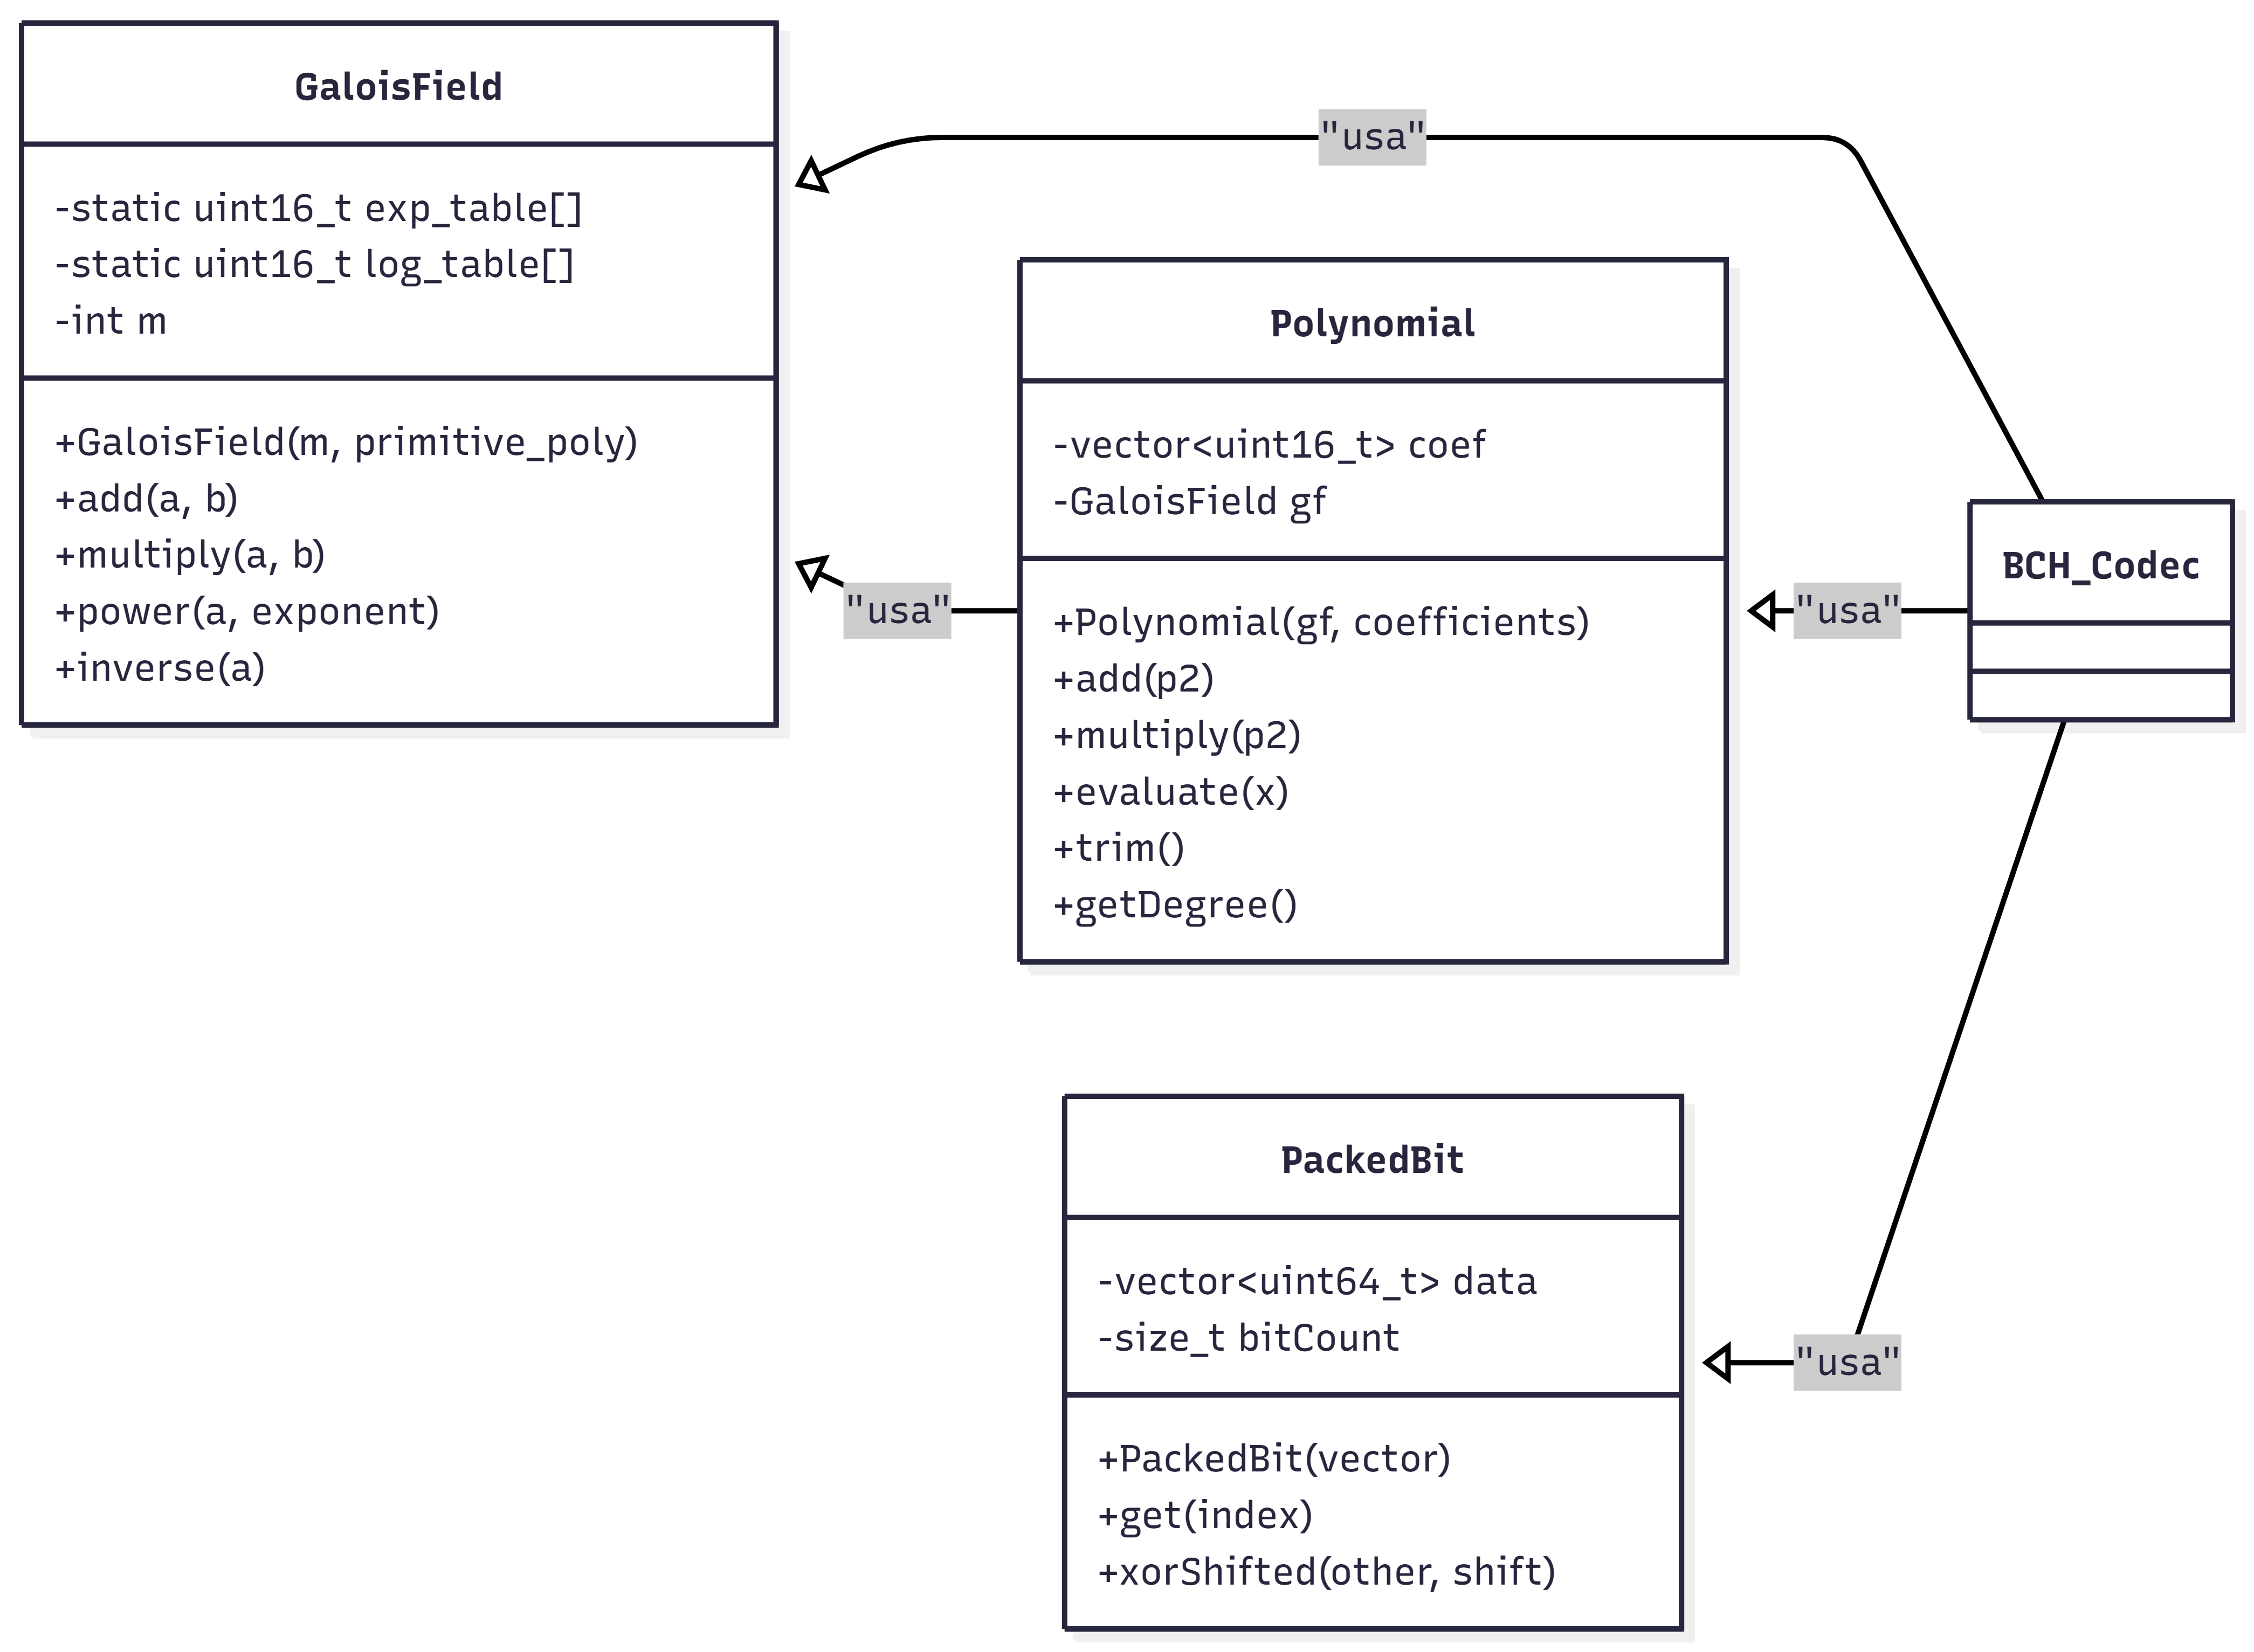
\includegraphics[width=0.95\textwidth]{../imagenes/UML_math.png}
    \caption{Diagrama UML del subsistema matemático.}
    \label{fig:uml_math}
\end{figure}

A continuación se describen las clases principales que lo componen:

\subsubsection{Clase \texttt{GaloisField}}

La clase \texttt{GaloisField} constituye el fundamento algebraico del simulador. Implementa la aritmética completa en el cuerpo finito $GF(2^m)$ mediante representación logarítmica/exponencial (tablas log/antilog).

\begin{itemize}
    \item \textbf{Construcción:} Recibe el grado $m$ y un polinomio primitivo irreducible. Calcula y almacena en tablas estáticas (\texttt{exp\_table} y \texttt{log\_table}) las potencias de un elemento primitivo.
    
    \item \textbf{Operaciones implementadas:} suma (XOR), multiplicación, división, inversa y potenciación, todas optimizadas mediante acceso a tablas.
    
    \item \textbf{Decisiones de diseño:}
        \begin{itemize}
            \item Tablas estáticas compartidas entre todas las instancias (se calculan una única vez por valor de $m$).
            \item Soporte hasta $m=15$ (límite práctico impuesto por \texttt{uint16\_t}).
            \item Polinomios primitivos predefinidos para cada $m$ soportado.
        \end{itemize}
\end{itemize}

\subsubsection{Clase \texttt{Polynomial}}

Representa polinomios sobre $GF(2^m)$. Se usan \texttt{vector<uint16\_t>} para almacenar los coeficientes, donde el índice corresponde al grado del monomio.

\begin{itemize}
    \item Métodos principales: \texttt{add()}, \texttt{multiply()}, \texttt{evaluate()} y \texttt{trim()}.
    \item El método \texttt{trim()} elimina coeficientes nulos de mayor grado, manteniendo el tamaño mínimo del vector.
    \item Uso principal: construcción del polinomio generador y evaluación de síndromes.
\end{itemize}

\subsubsection{Clase \texttt{PackedBit}}

Estructura optimizada para operaciones a nivel de bits. Almacena los bits empaquetados en bloques de 64 bits (\texttt{uint64\_t}).

Su operación más crítica es \texttt{xorShifted()}, utilizada en la división polinómica durante la codificación sistemática. Esta optimización aporta una mejora significativa de rendimiento respecto a la implementación vectorial original.

\subsection{Subsistema Códec BCH}
El núcleo del simulador se encuentra en la clase \texttt{BCH\_Codec}, que implementa toda la lógica específica de los códigos BCH (codificación sistemática y decodificación algebraica).

\begin{figure}[ht]
    \centering
    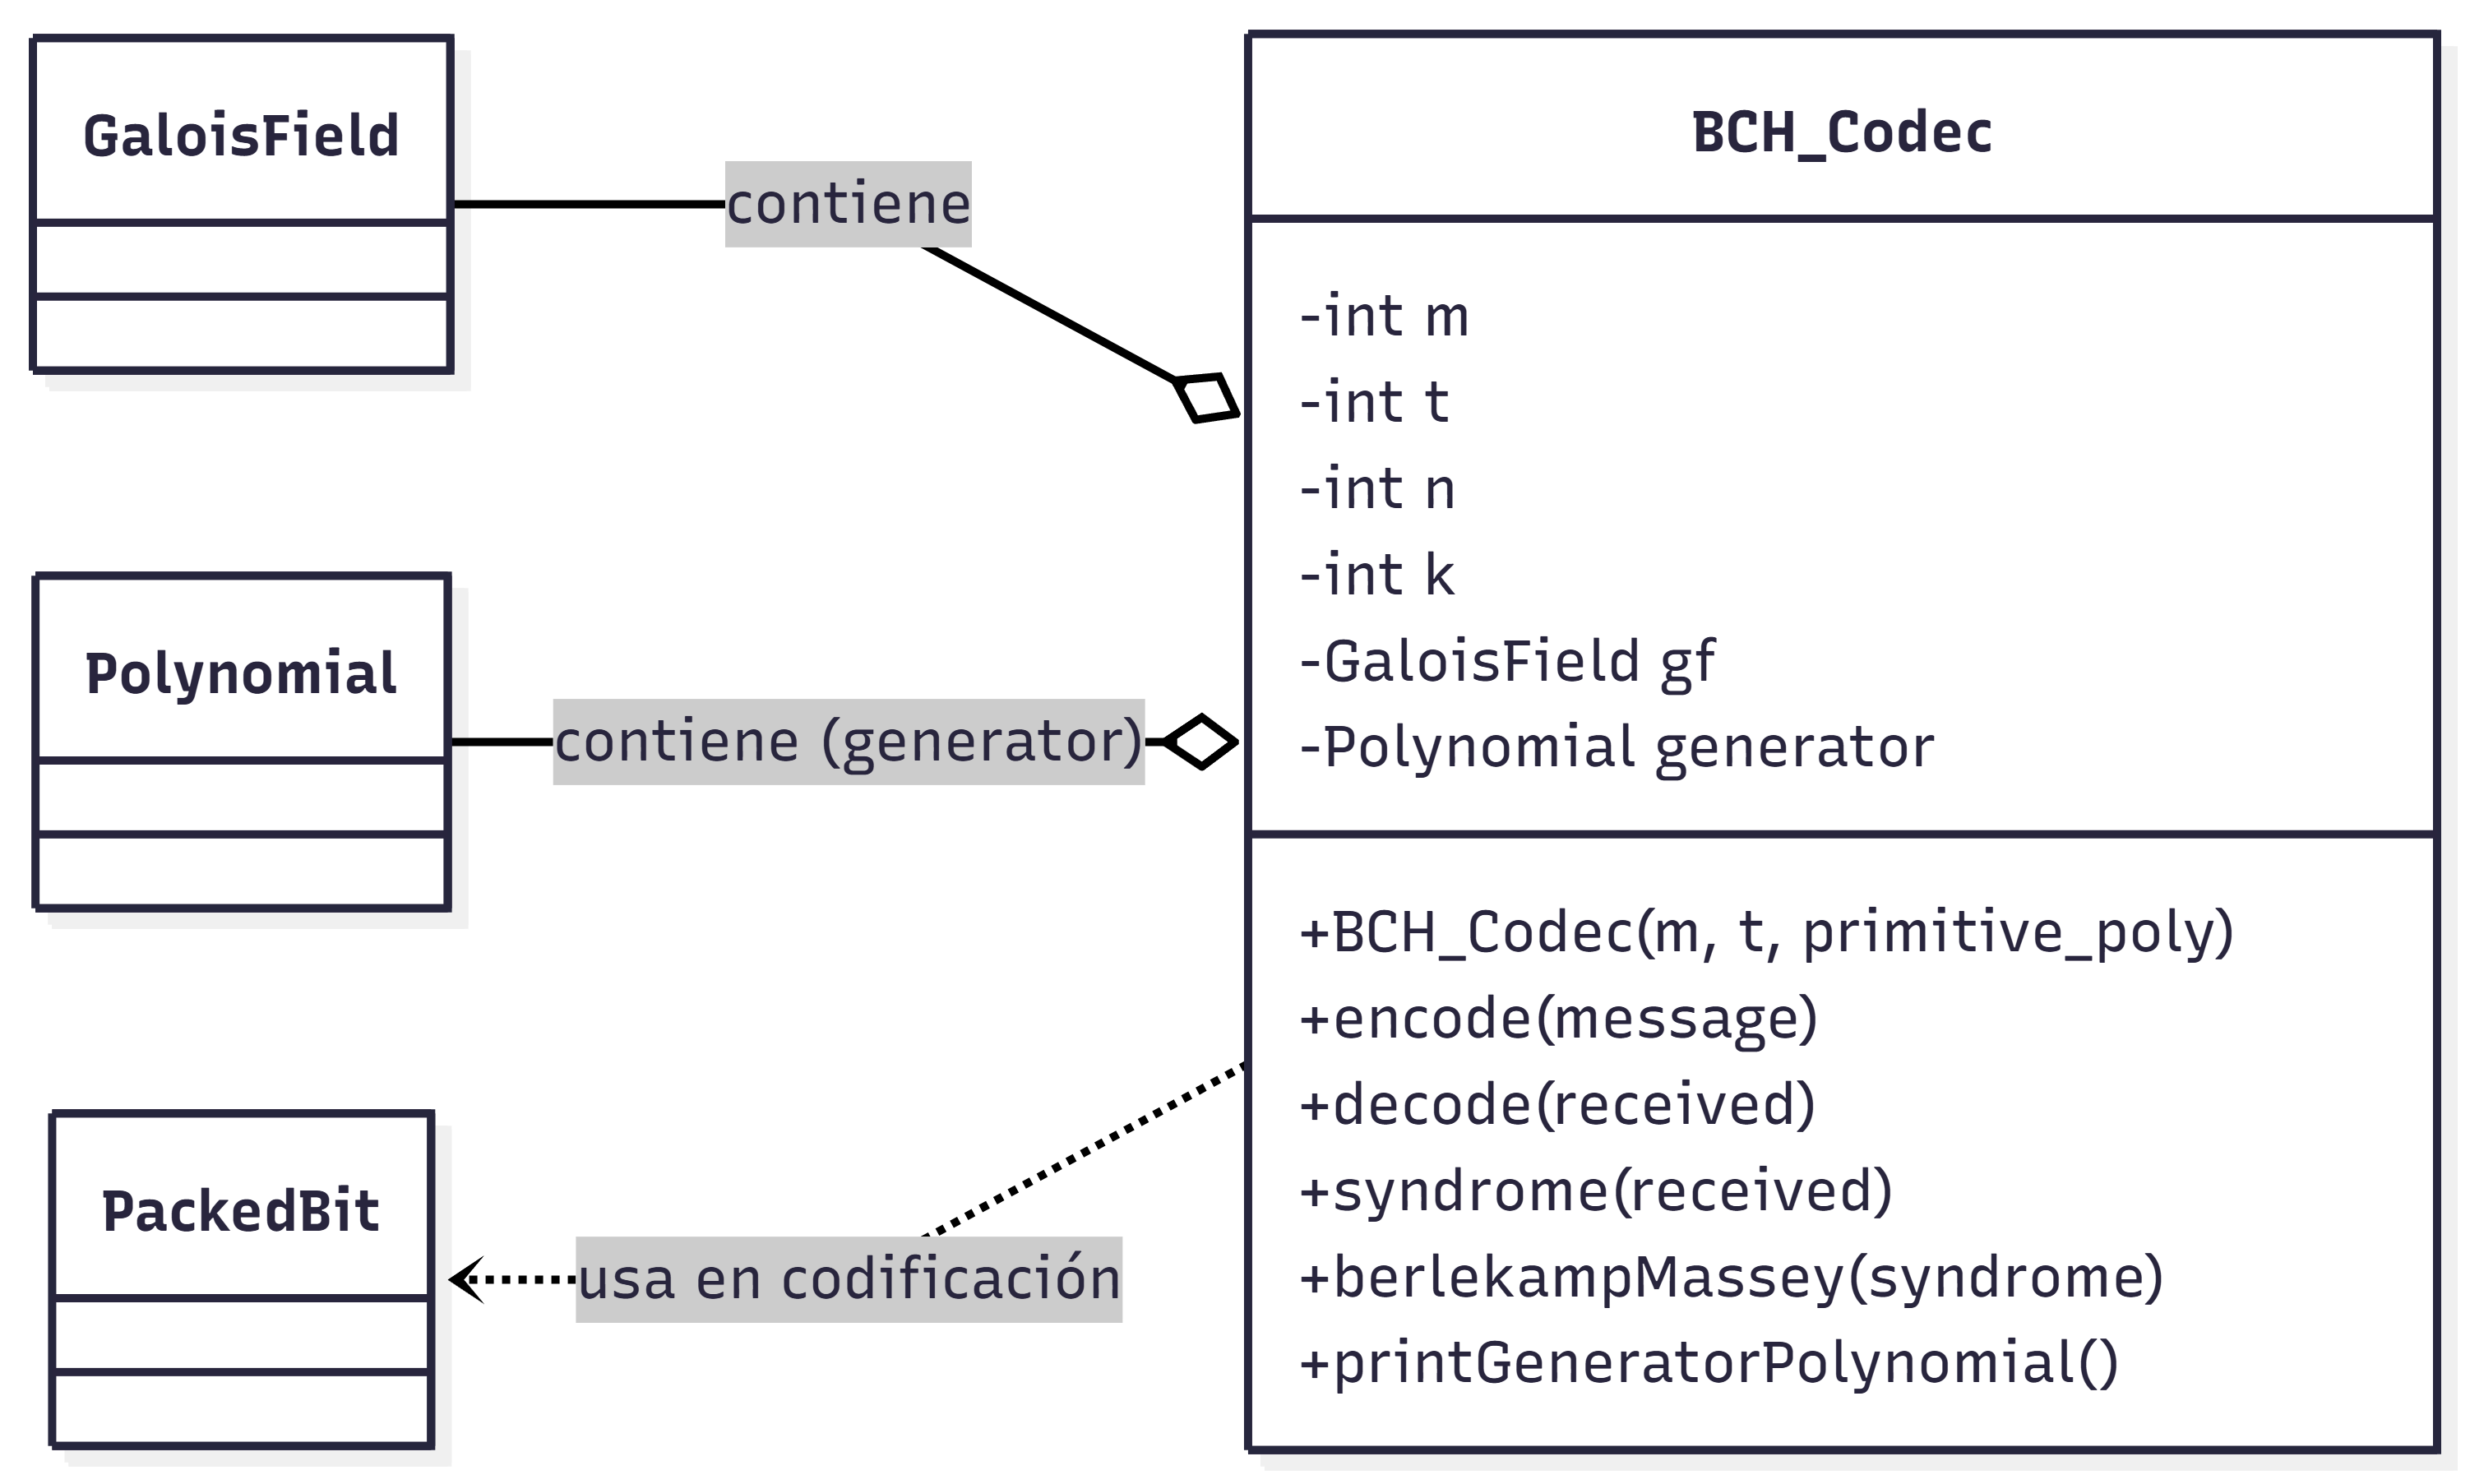
\includegraphics[width=0.95\textwidth]{../imagenes/UML_codec.png}
    \caption{Diagrama UML del subsistema Códec BCH.}
    \label{fig:uml_codec}
\end{figure}

A continuación se describen los detalles de su implementación:

\subsubsection{Clase \texttt{BCH\_Codec}}

Clase central que encapsula toda la lógica específica de los códigos BCH.

\begin{itemize}
    \item \textbf{Inicialización:}
    \begin{itemize}
        \item Calcula $n = 2^m - 1$.
        \item Construye el polinomio generador $g(x)$ multiplicando los polinomios mínimos correspondientes a las raíces $\alpha^1, \alpha^2, \dots, \alpha^{2t}$.
        \item Calcula automáticamente $k = n - \deg(g(x))$.
    \end{itemize}

    \item \textbf{Codificación sistemática:}
    Se implementaron y compararon dos estrategias:
    \begin{itemize}
        \item Versión basada en \texttt{PackedBit} (seleccionada finalmente por su superior rendimiento).
        \item Versión basada en registro de desplazamiento lineal (LFSR).
    \end{itemize}

    \item \textbf{Decodificación algebraica:}
    \begin{itemize}
        \item Cálculo de síndromes con optimización para índices pares ($S_{2i} = S_i^2$).
        \item Algoritmo de \textbf{Berlekamp-Massey} optimizado (trabajando directamente con vectores para reducir el \textit{overhead} de objetos \texttt{Polynomial}).
        \item Búsqueda de Chien para localizar y corregir hasta $t$ errores por palabra código.
    \end{itemize}
\end{itemize}

\subsection{Subsistema de Canal}

\subsubsection{Clase \texttt{Channel}}

Implementa los dos modelos de canal utilizados en las simulaciones:

\begin{itemize}
    \item \textbf{Canal Binario Simétrico (BSC):} Invierte cada bit de forma independiente con probabilidad $p$.
    \item \textbf{Canal AWGN con modulación BPSK y decisión dura:}
    \begin{itemize}
        \item Mapea los bits según la convención $0 \mapsto +1$ y $1 \mapsto -1$.
        \item Añade ruido gaussiano blanco aditivo con varianza calculada en función de $E_s/N_0$.
        \item Realiza decisión dura sobre la señal recibida.
    \end{itemize}
\end{itemize}

\subsection{Subsistema de Simulación y Orquestación}
Este subsistema es el responsable de coordinar todo el proceso de simulación Monte Carlo, gestionando la configuración, la paralelización y la recolección de resultados.

\begin{figure}[ht]
    \centering
    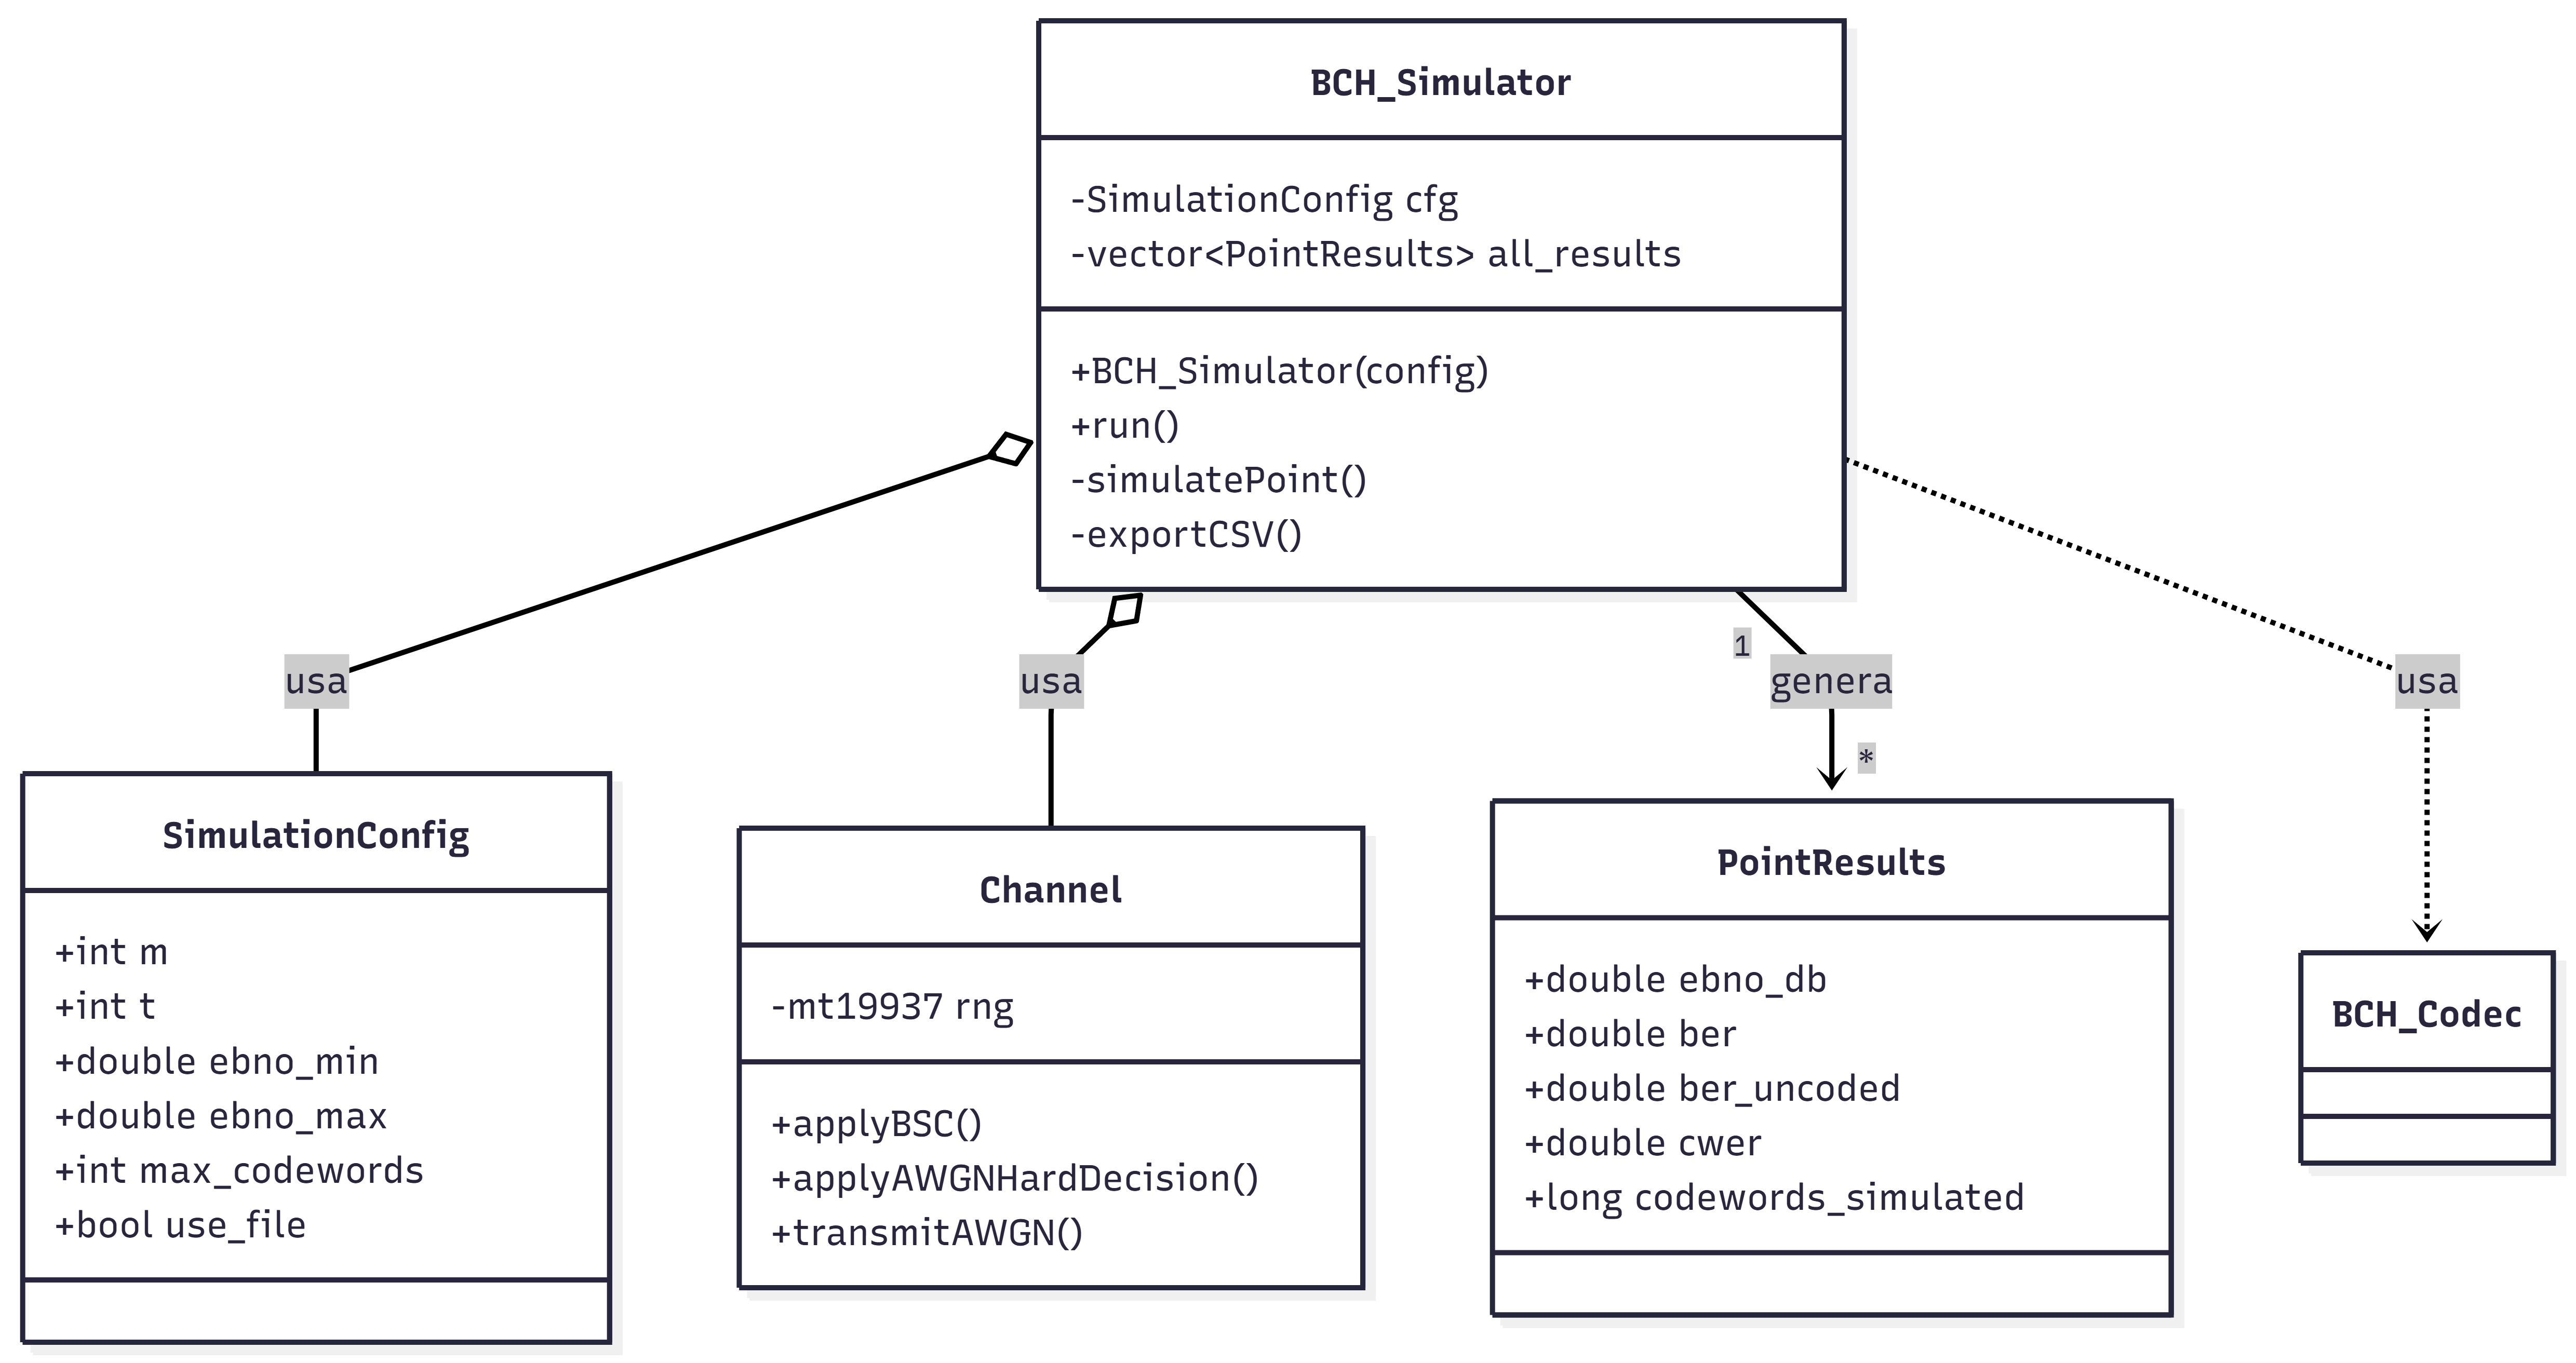
\includegraphics[width=0.95\textwidth]{../imagenes/UML_sim.png}
    \caption{Diagrama UML del subsistema de simulación y orquestación.}
    \label{fig:uml_sim}
\end{figure}

A continuación se detallan las clases principales:

\subsubsection{Clase \texttt{BCH\_Simulator}}

Es el orquestador principal del simulador. Su diseño separa la ejecución en dos flujos de trabajo gestionados por el método \texttt{run()}:
\begin{itemize}
    \item \textbf{Flujo Matemático (\texttt{simulatePoint}):} Dedicado exclusivamente a las simulaciones de Montecarlo. Emplea paralelización mediante OpenMP para evaluar el rendimiento estadístico del código frente a canales AWGN y recolectar métricas cuantitativas (BER, CWER, latencias).
    \item \textbf{Flujo Cualitativo (\texttt{processFile}):} Orientado a la demostración práctica con archivos reales. Este flujo también ha sido diseñado para operar en paralelo mediante OpenMP, procesando la totalidad del archivo como un flujo de datos en crudo para evaluar la robustez del código frente a la corrupción de la información.
    \item \textbf{Gestión de configuración y exportación:} Controla los criterios de parada, la orquestación del generador de pseudoaleatorios y la exportación de resultados a formato CSV.
\end{itemize}

\subsection{Decisiones de Diseño y Optimizaciones}

Las principales decisiones de diseño estuvieron orientadas a maximizar el rendimiento en simulaciones Monte Carlo:

\begin{itemize}
    \item Elección de C++ en lugar de Python o MATLAB por su cercanía al hardware y control de bajo nivel.
        \item Uso intensivo de optimizaciones (\texttt{PackedBit}, tablas estáticas).
    \item Paralelización con OpenMP en lugar de múltiples procesos para reducir overhead.
    \item Decodificación \textit{hard-decision} como compromiso entre complejidad y representatividad.
\end{itemize}

Estas decisiones permitieron ejecutar simulaciones con millones de palabras código en tiempos razonables, algo fundamental para obtener curvas BER/CWER confiables.